\documentclass{sig-alternate}

\conferenceinfo{ICMR}{'12, June 5--8, Hong Kong, China}
\CopyrightYear{\copyright 2012}
\crdata{978-1-4503-1329-2/12/06}

\usepackage[utf8]{inputenc}
\usepackage[T1]{fontenc}

\usepackage[activate=compatibility]{microtype}

% autoref command
\usepackage[pdftex,urlcolor=black,colorlinks=true,linkcolor=black,citecolor=black]{hyperref}
\def\sectionautorefname{Section}
\def\subsectionautorefname{Subsection}
\def\subfloatautorefname{Subfigure}

\usepackage[lofdepth,lotdepth]{subfig}

\usepackage{enumitem}

\usepackage{mathtools}

% give emph a normal fontsize
\let\oldemph\emph
\renewcommand{\emph}[1]{\oldemph{\fontsize{9}{9}\selectfont #1}}

% more readable footnote layout
\renewcommand{\footnotesize}{\fontsize{8pt}{10pt}}
\setlength{\footnotesep}{.5cm}

% todo macro
\usepackage{color}
\newcommand{\todo}[1]{\noindent\textcolor{red}{{\bf \{TODO}: #1{\bf \}}}}

% listings and Verbatim environment
\usepackage{fancyvrb}
\usepackage{relsize}
\usepackage{listings}
\usepackage{verbatim}
\newcommand{\defaultlistingsize}{\fontsize{8pt}{9.5pt}}
\newcommand{\inlinelistingsize}{\fontsize{8pt}{11pt}}
\newcommand{\smalllistingsize}{\fontsize{7.5pt}{9.5pt}}
\newcommand{\listingsize}{\defaultlistingsize}
\RecustomVerbatimCommand{\Verb}{Verb}{fontsize=\inlinelistingsize}
\RecustomVerbatimEnvironment{Verbatim}{Verbatim}{fontsize=\defaultlistingsize}
\lstset{frame=lines,captionpos=b,numberbychapter=false,escapechar=§,
        aboveskip=0.5em,belowskip=0em,abovecaptionskip=0em,belowcaptionskip=0em,
framexbottommargin=-1em,
        basicstyle=\ttfamily\listingsize\selectfont}

% use Courier from this point onward
\let\oldttdefault\ttdefault
\renewcommand{\ttdefault}{pcr}
\let\oldurl\url
\renewcommand{\url}[1]{\inlinelistingsize\oldurl{#1}}

% superscript for 1st, 2nd, etc.
\newcommand{\superscript}[1]{\ensuremath{^{\textrm{#1}}}}
\newcommand{\subscript}[1]{\ensuremath{_{\textrm{#1}}}}
\newcommand{\th}[0]{\superscript{th}}
\newcommand{\st}[0]{\superscript{st}}
\newcommand{\nd}[0]{\superscript{nd}}
\newcommand{\rd}[0]{\superscript{rd}}

% linewrap symbol
\definecolor{grey}{RGB}{130,130,130}
\newcommand{\linewrap}{\raisebox{-.6ex}{\textcolor{grey}{$\hookleftarrow$}}}

% more pleasing quote environment
\usepackage{tikz}
\newcommand*{\openquote}{\tikz[remember picture,overlay,xshift=-7pt,yshift=1pt]
     \node (OQ) {\fontfamily{fxl}\fontsize{16}{16}\selectfont``};\kern0pt}
\newcommand*{\closequote}{\tikz[remember picture,overlay,xshift=2pt,yshift=-4.5pt]
     \node (CQ) {\fontfamily{fxl}\fontsize{16}{16}\selectfont''};}
\renewenvironment{quote}%
{\setlength{\parindent}{1cm}\par\openquote}
{\closequote\vspace{-4.5pt}
}

\begin{document}

\title{One Size Does Not Fit All -- Multimodal Search on Mobile and Desktop Devices with the \mbox{I-SEARCH} Search Engine}

\numberofauthors{17}
\author{
\alignauthor
Thomas Steiner\\
	\affaddr{Google Germany GmbH}\\
	\email{tomac@google.com}
\alignauthor
Lorenzo Sutton\\
	\affaddr{Accademia Naz. di S. Cecilia}\\
	\email{l.sutton@santacecilia.it}
\alignauthor
Sabine Spiller\\ 	
	\affaddr{EasternGraphics GmbH}\\
	\email{spiller@easterngraphics.com}
\and	
\alignauthor	
Marilena Lazzaro, Francesco Nucci, and Vincenzo Croce\\
	\affaddr{Engineering}\\
	\email{\{first.last\}@eng.it}
\alignauthor
Alberto Massari, and Antonio Camurri\\
	\affaddr{University of Genova}\\
	\email{alby@infomus.dist.unige.it, antonio.camurri@unige.it}  
\alignauthor	
Anne Verroust-Blondet, and Laurent Joyeux\\
	\affaddr{INRIA Rocquencourt}\\
	\email{\{anne.verroust, laurent.joyeux\}@inria.fr}
}

\additionalauthors{Additional authors:
Jonas Etzold, Paul Grimm
(Hochschule Fulda,
email: \texttt{\{jonas.etzold, paul.grimm\}@hs-fulda.de}),
Athanasios Mademlis, Sotiris Malassiotis, Petros Daras, Apostolos Axenopoulos, Dimitrios Tzovaras
(CERTH/ITI,
email: \texttt{\{mademlis, malasiot, daras, axenop, tzovaras\}@iti.gr})
}

\maketitle

\begin{abstract}
In this paper, we report on work around the \mbox{I-SEARCH} EU (FP7 ICT STREP) project whose objective is the development of a multimodal search engine targeted at mobile and desktop devices.
Each of these device classes has its specific hardware capabilities and set of supported features.
In order to provide a common multimodal search experience across device classes, one size does not fit all.
We highlight ways to achieve the same functionality agnostic of the device class being used for the search, and present concrete use cases.
\end{abstract}

\category{H.3.4}{Information Systems}{Information Storage and Retrieval}[World Wide Web]
%\category{H.3.5}{Online Information Services}{Web-based services}

\terms{Experimentation}

\keywords{Multimodality, Rich Unified Content Description, IR}

\section{Introduction} \label{sec:introduction}
Even in 2012, search is a mainly text-driven operation.
Albeit recent developments in the mobile and desktop worlds have introduced voice search as an \emph{additional} input modality, a \emph{truly multimodal} search experience with multimodal in- and output is still missing.
In the scope of \mbox{I-SEARCH}, industrial and academic partners are working together to investigate ways to provide such a multimodal search experience across device classes.
We provide an overview of the project in its entirety in~\cite{www2012}.
An important step towards multimodal search in the scope of \mbox{I-SEARCH} was the creation of a unified annotation format named \emph{Rich Unified Content Description (RUCoD)}, which was detailed in~\cite{ijmis2010}.

In this paper, we focus on taken actions and future plans to deal with device constraints to support the in- and output modalities \emph{audio}, \emph{video}, \emph{rhythm}, \emph{image}, \emph{3D object}, \emph{sketch}, \emph{emotion}, \emph{geolocation}, and \emph{text}.
The \mbox{I-SEARCH} project is in its second year now, and some basic functionality is in place.
We maintain a demonstration server\footnote{Demonstration: \url{http://isearch.ai.fh-erfurt.de/}}, and have also recorded a screencast\footnote{Screencast: \url{http://youtu.be/-chzjEDcMXU}} showing features of the search engine.

\section{User-facing Project Goals} \label{sec:projectgoals}
\mbox{I-SEARCH} is a complex project that touches on many research areas treated by the different project partners.
One important goal is to hide this complexity from the end user through a consistent and context-aware user interface based on standard HTML5, JavaScript, and CSS, with ideally no additional plug-ins like Flash required.
We aim at sharing one common code base for both device classes, mobile and desktop, with the user interface getting progressively enhanced~\cite{progressiveenhancement} the more capable the user's Web browser and connection speed are.
The user interface presentation can be tailored to a specific range of output devices without changing the content itself by using CSS3 Media Queries~\cite{mediaqueries}.
Search engines over the years have coined a common interaction pattern: the search box.
We enhance this interaction pattern by context-aware modality input toggles that create modality query tokens in the \mbox{I-SEARCH} search box.
\autoref{fig:ui} shows three example modality query tokens for \emph{audio}, \emph{emotion}, and \emph{geolocation}.

\begin{figure}
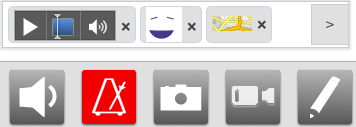
\includegraphics[width=\columnwidth]{./resources/ui.png}
\caption{\mbox{I-SEARCH} search box with three modality query tokens for \emph{audio}, \emph{emotion}, and \emph{geolocation}.}
\label{fig:ui}
\vspace{-0.9em}
\end{figure}

\section{Use Cases} \label{sec:usecases}
In order to give the reader an idea of intended \mbox{I-SEARCH} usage and to motivate multimodality, we introduce three use cases and involved modalities as defined by the project.
%\vspace{-1.5em}

\paragraph{UC1: Music Expert (Desktop, Mobile)}
A music expert with access to a big music archive does research on the influence of traditional folk music on today's popular music.
She inputs a \emph{rhythm} to the \mbox{I-SEARCH} system in order to search the archive for similar rhythm patterns.
She refines her query by adding \emph{geolocation} to limit results to a certain region and by uploading a disco \emph{image}.
%\vspace{-1.5em}

\paragraph{UC2: Interior Designer (Desktop)}
An interior designer wants to give her client a realistic idea of office chairs.
She uploads a \emph{3D model} of a chair that almost matches her client's expectations to the \mbox{I-SEARCH} system, together with an \emph{image} of the upholstery.
She refines with a hand-drawn \emph{sketch} of the chair's shape.
%\vspace{-1.5em}

\paragraph{UC3: World Traveler (Mobile)}
A traveler uses her cell phone with the \mbox{I-SEARCH} app to create media content with associated \emph{geolocation} data like \emph{videos} and \emph{images} of the sights she visits to retrieve related content of other travelers, \emph{text} descriptions, and \emph{3D models} that she wants to use to map her trip on a virtual globe.

\section{Modalities Across Devices}
In this Section, we focus on \emph{input} modalities across \emph{mobile} and \emph{desktop} device classes and their support in \mbox{I-SEARCH}.\\

\noindent \textbf{Audio, Image, Video}
We describe audio, image, and video modalities together, as they share the same interaction patterns.
On desktop devices, audios, images, or videos can be uploaded from the user's hard disk via a file upload dialog or via drag 'n' drop.
On some mobile devices (e.g., iOS devices) file uploading is prohibited, which is why in the longterm, as support advances, we aim at using the getUserMedia API~\cite{getusermedia}.
At time of writing, access to getUserMedia is available in developer
preview builds of several browsers.
The fallback solution is a Flash uploader.\\
%\vspace{-1.5em}

\noindent \textbf{Rhythm}
On desktop devices, we support entering a rhythm by key presses or mouse tapping, whereas additionally on mobile devices a rhythm can also be captured via the device orientation API~\cite{deviceorientation} by tilting the device rhythmically.\\
%\vspace{-1.5em}

\noindent \textbf{3D Object}
We support 3D objects on mobile and desktop via the COLLADA 3D asset exchange schema~\cite{collada}.
3D objects can be inserted via a file upload dialog or drag 'n' drop.\\ 
%\vspace{-1.5em}

\noindent \textbf{Text}
On mobile and desktop, text can be entered using the keyboard or using the speech input API~\cite{speechinput}.\\

\noindent \textbf{Emotion}
In order to accompany a query by basic emotional feedback, we have adapted an open-source emotion input solution~\cite{emotionslider} for mobile and desktop that transfers the slider user interface pattern to emotions from sad to happy.\\ 
%\footnote{\url{http://glittle.org/smiley-slider/}}
%\vspace{-1.5em}

\noindent \textbf{Geolocation}
For retrieving and tracking a user's physical location, we use the HTML5 geolocation API~\cite{geolocation}, which is available in Web browsers on mobile and desktop devices.\\
%\vspace{-1.5em}

\noindent \textbf{Sketch}
Hand-drawn sketches can be created on mobile and desktop devices alike using a simple touch-based HTML5 canvas~\cite{canvas} sketch editor.
%\vspace{-1.5em}

\section{Future Work and Conclusion}
We have introduced the \mbox{I-SEARCH} project and three of its use cases and have shown how different input modalities are supported on mobile and desktop. Now we need to integrate the project partners' services in the back-end, in order to support multimodal output besides multimodal input.

\section{Acknowledgments}
This work was partially supported by the European Commission under Grant No. 248296 FP7 \mbox{I-SEARCH} project.

% back to normal size Computer Modern for URLs in bibliography
\let\ttdefault\oldttdefault
\let\url\oldurl

% decrease space between bibliographic references
\let\oldbibitem\bibitem
\renewcommand{\bibitem}[1]{%
	\ifx\bibstarted\undefined
		\def\bibstarted{1}
		\vspace{.1em}
	\else
		\vspace{-.2em plus .1em minus .1em}
	\fi
\oldbibitem{#1}}

\bibliographystyle{abbrv}
\bibliography{icmr2012}

\balancecolumns
\end{document}